%-----------------------------------------------------------------------------
% Author: Rayla Kurosaki
% GitHub: https://github.com/rkp1503
%-----------------------------------------------------------------------------
\documentclass{rayla-project}
\usepackage{rayla-math-style}

%-----------------------------------------------------------------------------
% Assignment Information
%-----------------------------------------------------------------------------
\myUniversity{
    Rochester Institute of Technology\\
    College of Science\\
    School of Physics and Astronomy
    }
\myTitle{Chaotic Behavior of Double Pendulum Systems}
\myName{Ramsey (Rayla) Phuc}
\courseid{PHYS-377.01}
\courseName{Advanced Computational Physics}
\professorName{Dr. Pratik Dholabhai}
\term{2021/01/25 - 2021/05/05}
\dueDate{2021/05/04}

%-----------------------------------------------------------------------------
% Start of Document
%-----------------------------------------------------------------------------
\begin{document}

    \maketitle

    %-------------------------------------------------------------------------
    % Abstract
    %-------------------------------------------------------------------------
    \begin{abstract}
        The double pendulum is a classic example of a chaotic system that exhibits complex and unpredictable behavior.
        In this paper, we investigate the dynamics of the double pendulum and analyze its chaotic characteristics.
        We begin by formulating the equations of motion using Lagrangian mechanics, considering the gravitational forces and constraints on the system.
        Through numerical simulations and computational techniques, we explore the evolution of the double pendulum system under various initial conditions.
        Our analysis reveals that the double pendulum demonstrates sensitive dependence on initial conditions, commonly referred to as the ``butterfly effect''.
        Small variations in the initial conditions lead to significant deviations in the system's subsequent motion, making long-term predictions challenging.
    \end{abstract}

    %-------------------------------------------------------------------------
    % Body
    %-------------------------------------------------------------------------
    \section{Introduction and Background}
\subsection{Introduction}
A dynamical system, in physics, typically describes the state of a particle that varies over time. One particular example of a dynamical system in physics is the double pendulum. A single pendulum consists of one object (a bob) that is connected to a fixed point by an non-stretchable string. A double pendulum is an extension of the single pendulum where you attach another bob at the end of the single pendulum. Unlike a single pendulum, the double pendulum has a strong sensitivity to its initial conditions, which causes the double pendulum to behave in a chaotic way. 

\subsection{Goals}
\begin{enumerate}
    \item Derive the potential, kinetic, and total energies of a generic double pendulum system.
    \item Derive the system of equations that represents the motion for a generic double pendulum system.
    \item Solve the system of equations numerically using a custom ODE solver. This solver uses the Runge-Kutta Order 4 method.
    \item Create an animation of the double pendulum along with some animated graphs. These animated graphs are meant to be in sync with the double pendulum animation.
    \item Show that the Double Pendulum system is a chaotic system by showing the differences a small change in a initial condition can do.
\end{enumerate}

\subsection{Fundamental Physics}
Figure~\ref{fig:1} captures a frame of the double pendulum. Here we will set the initial anchor at the origin $O$. $x_i$ represents the horizontal distance from the origin to bob $i$, $y_i$ represents the vertical distance from the origin to bob $i$, and $\theta_i$ represents the angle bob $i$ makes between the anchor or the bob above it and the vertical. \\

We can derive the equations that are necessary to show the behavior of this chaotic system. Lets start by deriving the potential, kinetic, and the total energy of this system. From Figure~\ref{fig:1}, we can determine the positions of each bob. The $x$ and $y$ coordinates for bob 1 are:

\begin{equation}
    \begin{aligned}
        x_1 &= l_1\sin\left(\theta_1\right)\\
        y_1 &= -l_1\cos\left(\theta_1\right)
    \end{aligned}
    \label{eq:bob-1-position-components}
\end{equation}

and the $x$ and $y$ coordinates for bob 2 are:

\begin{equation}
    \begin{aligned}
        x_2 &= l_1\sin\left(\theta_1\right) + l_2\sin\left(\theta_2\right)\\
        y_2 &= -l_1\cos\left(\theta_1\right) - l_2\cos\left(\theta_2\right)
    \end{aligned}
    \label{eq:bob-2-position-components}
\end{equation}

Next, we will compute the total potential energy of the system. We know that the potential energy for bob $i$ is $PE_i = m_i g h_i$. We also know that $h_i$ is the vertical component of bob $i$, or $y_i$. Using these $y$ components from Equations (\ref{eq:bob-1-position-components})-(\ref{eq:bob-2-position-components}), we can compute the total potential energy of the system:

\begin{align*}
    PE &= PE_1 + PE_2\\
    PE &= m_1gh_1 + m_2gh_2\\
    PE &= m_1gy_1 + m_2gy_2\\
    PE &= m_1g\left(-l_1\cos\left(\theta_1\right)\right) + m_2g\left(-l_1\cos\left(\theta_1\right) - l_2\cos\left(\theta_2\right)\right)
\end{align*}

or 

\begin{equation}
    PE = -\left(m_1 + m_2\right)gl_1\cos\left(\theta_1\right) - m_2gl_2\cos\left(\theta_2\right)
    \label{eq:potential-energy}
\end{equation}

Next, we will compute the first time derivatives of the equations in Equation~\ref{eq:bob-1-position-components} to get bob 1's velocity components:

\begin{equation}
    \begin{aligned}
        v_{x_1} &= l_1\dot{\theta_1}\cos\left(\theta_1\right)\\
        v_{y_1} &= l_1\dot{\theta_1}\sin\left(\theta_1\right)
    \end{aligned}
    \label{eq:bob-1-velocity-components}
\end{equation}

Repeating this procedure on Equation~\ref{eq:bob-2-position-components} for bob 2 yields:

\begin{equation}
    \begin{aligned}
        v_{x_2} &= l_1\dot{\theta_1}\cos\left(\theta_1\right) + l_2\dot{\theta_2}\cos\left(\theta_2\right)\\
        v_{y_2} &= l_1\dot{\theta_1}\sin\left(\theta_1\right) + l_2\dot{\theta_2}\sin\left(\theta_2\right)
    \end{aligned}
    \label{eq:bob-2-velocity-components}
\end{equation}

We know that the velocity of bob $i$ is $v_i^2 = v_{x_i}^2 + v_{y_i}^2$. Using the equations in Equation~\ref{eq:bob-1-velocity-components}, we can compute the velocity of bob 1:

\begin{equation}
    v_1^2 = l_1^2\dot{\theta_1}^2
    \label{eq:bob-1-velocity}
\end{equation}

And we can follow the same steps to compute the velocity of bob 2:

\begin{equation}
    v_2^2 = l_1^2\dot{\theta_1}^2 + l_2^2\dot{\theta_2}^2 + 2l_1l_2\dot{\theta_1}\dot{\theta_2}\cos\left(\theta_1 - \theta_2\right)
    \label{eq:bob-2-velocity}
\end{equation}

With this, we can now compute the total kintetic energy of the system. We know that the kinetic energy for bob $i$ is $KE_i = \left(m_i v_i^2\right)/2$. With Equations (\ref{eq:bob-1-velocity})-(\ref{eq:bob-2-velocity}), we can say that the total kinetic energy of the system is:

\begin{align*}
    KE &= KE_1 + KE_2\\
    KE &= \frac{m_1 v_1^2}{2} + \frac{m_2 v_2^2}{2}\\
    KE &= \frac{m_1 \left(l_1^2\dot{\theta_1}^2\right)}{2} + \frac{m_2 \left(l_1^2\dot{\theta_1}^2 + l_2^2\dot{\theta_2}^2 + 2l_1l_2\dot{\theta_1}\dot{\theta_2}\cos\left(\theta_1 - \theta_2\right)\right)}{2}
\end{align*}

or:

\begin{equation}
    KE = \frac{\left(m_1 + m_2\right)l_1^2\dot{\theta_1}^2+m_2l_2^2\dot{\theta_2}^2}{2} + m_2l_1l_2\dot{\theta_1}\dot{\theta_2}\cos\left(\theta_1 - \theta_2\right)
    \label{eq:kinetic-energy}
\end{equation}

With expressions for the total potential energy and the total kinetic energy, we can compute the total energy of the system. The total energy is the sum of all energies. Thus, we have $TE=KE+PE$ or:

\begin{equation}
    TE = \frac{\left(m_1 + m_2\right)l_1^2\dot{\theta_1}^2+m_2l_2^2\dot{\theta_2}^2}{2} + m_2l_1l_2\dot{\theta_1}\dot{\theta_2}\cos\left(\theta_1 - \theta_2\right) - \left(m_1 + m_2\right)gl_1\cos\left(\theta_1\right) - m_2gl_2\cos\left(\theta_2\right)
    \label{eq:total-energy}
\end{equation}

Now lets derive the equations that capture the motion of the system. To do this, we will need to determine the Lagrangian. The lagrangian of a system is $L=KE-PE$. For this system, the lagrangian is:

\begin{equation}
    L = \frac{\left(m_1 + m_2\right)l_1^2\dot{\theta_1}^2+m_2l_2^2\dot{\theta_2}^2}{2} + m_2l_1l_2\dot{\theta_1}\dot{\theta_2}\cos\left(\theta_1 - \theta_2\right) + \left(m_1 + m_2\right)gl_1\cos\left(\theta_1\right) + m_2gl_2\cos\left(\theta_2\right)
    \label{eq:lagrangian}
\end{equation}

Now we will need to utilize the Euler-Lagrange equation, which states:

\begin{equation}
    \diff[]{}{t}\left(\pdiff[]{L}{\dot{\theta}}\right) - \pdiff[]{L}{\theta} = 0
    \label{eq:euler-lagrange}
\end{equation}

We will apply the Euler-Lagrange equation to both $\theta_1$ and $\theta_2$. Applying the Euler-Lagrange equation to $\theta_1$, we get:

\begin{align*}
    0 &= \diff[]{}{t}\left(\pdiff[]{L}{\dot{\theta_1}}\right) - \pdiff[]{L}{\theta_1}\\
    0 &= \diff[]{}{t}\left(\left(m_1 + m_2\right)l_1^2\dot{\theta_1} + m_2l_1l_2\dot{\theta_2}\cos\left(\theta_1 - \theta_2\right)\right) - \left(-m_2l_1l_2\dot{\theta_1}\dot{\theta_2}\sin\left(\theta_1 - \theta_2\right) - gl_1\left(m_1 + m_2\right)\sin\left(\theta_1\right)\right)\\
    0 &= \left(m_1 + m_2\right)l_1^2\ddot{\theta_1} + m_2l_1l_2\ddot{\theta_2}\cos\left(\theta_1 - \theta_2\right) + m_2l_1l_2\dot{\theta_1}\dot{\theta_2}\sin\left(\theta_1 - \theta_2\right) + gl_1\left(m_1 + m_2\right)\sin\left(\theta_1\right)
\end{align*}

or:

\begin{equation}
    \left(m_1 + m_2\right)l_1\ddot{\theta_1} + m_2l_2\ddot{\theta_2}\cos\left(\theta_1 - \theta_2\right) + m_2l_2\dot{\theta_1}\dot{\theta_2}\sin\left(\theta_1 - \theta_2\right) + g\left(m_1 + m_2\right)\sin\left(\theta_1\right) = 0
    \label{eq:bob-1-motion}
\end{equation}

Applying the Euler-Lagrange equation to $\theta_2$, we get:

\begin{align*}
    0 &= \diff[]{}{t}\left(\pdiff[]{L}{\dot{\theta_2}}\right) - \pdiff[]{L}{\theta_2}\\
    0 &= \diff[]{}{t}\left(m_2l_2^2\dot{\theta_2} + m_2l_1l_2\dot{\theta_1}\cos\left(\theta_1 - \theta_2\right)\right) - \left(m_2l_1l_2\dot{\theta_1}\dot{\theta_2}\sin\left(\theta_1 - \theta_2\right) - m_2gl_2\sin\left(\theta_2\right)\right)\\
    0 &= m_2l_2^2\ddot{\theta_2} + m_2l_1l_2\ddot{\theta_1}\cos\left(\theta_1 - \theta_2\right) - m_2l_1l_2\dot{\theta_1}\dot{\theta_2}\sin\left(\theta_1 - \theta_2\right) + m_2gl_2\sin\left(\theta_2\right)\\
    0 &= l_2\ddot{\theta_2} + l_1\ddot{\theta_1}\cos\left(\theta_1 - \theta_2\right) - l_1\dot{\theta_1}\dot{\theta_2}\sin\left(\theta_1 - \theta_2\right) + g\sin\left(\theta_2\right)
\end{align*}

or:

\begin{equation}
    l_2\ddot{\theta_2} + l_1\ddot{\theta_1}\cos\left(\theta_1 - \theta_2\right) - l_1\dot{\theta_1}\dot{\theta_2}\sin\left(\theta_1 - \theta_2\right) + g\sin\left(\theta_2\right) = 0
    \label{eq:bob-2-motion}
\end{equation}

We will now combine Equations (\ref{eq:bob-1-motion}) and (\ref{eq:bob-2-motion}) to create a system of equations:

\begin{equation*}
    \begin{dcases}
        \begin{aligned}
            0 &= \left(m_1 + m_2\right)l_1\ddot{\theta_1} + m_2l_2\ddot{\theta_2}\cos\left(\theta_1 - \theta_2\right) + m_2l_2\dot{\theta_1}\dot{\theta_2}\sin\left(\theta_1 - \theta_2\right) + g\left(m_1 + m_2\right)\sin\left(\theta_1\right)\\
            0 &= l_2\ddot{\theta_2} + l_1\ddot{\theta_1}\cos\left(\theta_1 - \theta_2\right) - l_1\dot{\theta_1}\dot{\theta_2}\sin\left(\theta_1 - \theta_2\right) + g\sin\left(\theta_2\right)
        \end{aligned}
    \end{dcases}
\end{equation*}

We can rewrite the above system of equations to express $\ddot{\theta}_1$ and $\ddot{\theta}_2$ with respect to the other variables and parameters:

\begin{equation*}
    \begin{dcases}
        \begin{aligned}
            \ddot{\theta}_1 &= \frac{-g\left(2m_1 + m_2\right)\sin\left(\theta_1\right) - m_2g\sin\left(\theta_1 - 2\theta_2\right) - 2m_2\left(\dot{\theta}_2^2l_2 + \dot{\theta}_1^2l_1\cos\left(\theta_1 - \theta_2\right)\right)\sin\left(\theta_1 - \theta_2\right)}{l_1\left(2m_1 + m_2 - m_2\cos\left(2\left(\theta_1 - \theta_2\right)\right)\right)}\\
            \ddot{\theta}_2 &= \frac{2\left(\dot{\theta}_1^2l_1\left(m_1 + m_2\right)+\left(m_1 + m_2\right)g\cos\left(\theta_1\right) + \dot{\theta}_2^2l_2m_2\cos\left(\theta_1 - \theta_2\right)\right)\sin\left(\theta_1 - \theta_2\right)}{l_2\left(2m_1 + m_2 - m_2\cos\left(2\left(\theta_1 - \theta_2\right)\right)\right)}
        \end{aligned}
    \end{dcases}
\end{equation*}

Finally, we can modify the system once more. We will let $\omega_i=\dot{\theta}_i$ to obtain a system of 4 ordinary differential equations:

\begin{equation}
    \begin{dcases}
        \begin{aligned}
            \dot{\theta}_1 &= \omega_1\\
            \dot{\theta}_2 &= \omega_2\\
            \dot{\omega}_1 &= \frac{-g\left(2m_1 + m_2\right)\sin\left(\theta_1\right) - m_2g\sin\left(\theta_1 - 2\theta_2\right) - 2m_2\left(\omega_2^2l_2 + \omega_1^2l_1\cos\left(\theta_1 - \theta_2\right)\right)\sin\left(\theta_1 - \theta_2\right)}{l_1\left(2m_1 + m_2 - m_2\cos\left(2\left(\theta_1 - \theta_2\right)\right)\right)}\\
            \dot{\omega}_2 &= \frac{2\left(\omega_1^2l_1\left(m_1 + m_2\right)+\left(m_1 + m_2\right)g\cos\left(\theta_1\right) + \omega_2^2l_2m_2\cos\left(\theta_1 - \theta_2\right)\right)\sin\left(\theta_1 - \theta_2\right)}{l_2\left(2m_1 + m_2 - m_2\cos\left(2\left(\theta_1 - \theta_2\right)\right)\right)}
        \end{aligned}
    \end{dcases}
    \label{eq:system-of-equations}
\end{equation}

    \section{Program Manual}\label{sec:program-manual}

\subsection{Summary of the program}\label{subsec:summary-of-the-program}
This program can be executed in two ways. You can either run the Jupyter Notebook file \texttt{main.ipynb} or run the python script \texttt{main.py}. Both files will generate the same output. The purpose of this program is to not only solve the equations of motion of the double pendulum system, but also generate an animation of a double pendulum system with different animated plots that are in sync with animation of the double pendulum system.

\subsection{Installation requirements}\label{subsec:installation-requirements}
For this program to work, you need to be able to successfully run a Jupyter Notebook or a Python file. The rest of this subsection assumes you have the ability to open, edit, and run a Jupyter Notebook or a Python file. The required libraries you need in order to successfully run the program are \texttt{matplotlib} and \texttt{numpy}. 

\subsection{Details on the program}\label{subsec:details-on-the-program}
After the user has decided on the value of the initial conditions and the parameters, the user can run the program. Upon running the program, the first thing that the program will do is solve the system of equations in \eqref{eq:system-of-equations}. The python code that captures the system of equations can be found in \appref{subsec:system-of-ordinary-differential-equations}. The method I used to solve this system of differential equations is the Runge-Kutta order 4 method. My implementation of this method can be found in \appref{subsec:my-implementation-of-the-runge-kutta-order-4-method}. The code in \appref{subsec:my-implementation-of-the-runge-kutta-order-4-method} has a function called \verb|get_data()|. The purpose of this helper function is to gather the data we want more easily. The input is an $n \times m$ array and it transposes that array. \appref{subsec:get-data-helper-function} shows the code for the function \verb|get_data()|. Once the system of differential equations is solved, the program will generate five plots based the solution to the system of differential equations. These five plots will be saved as images for the user's reference and they are plotting:

\begin{enumerate}
    \item $\theta_2$ vs $\theta_1$
    \item $\omega_2$ vs $\omega_1$
    \item $\theta_1, \theta_2$ vs time
    \item $\omega_1, \omega_2$ vs time
    \item Potential, Kinetic, and Total Energies vs time
\end{enumerate}

After the plots are generated and saved as images, the program will create an animation. Using the constants, parameters, and initial conditions that the user initialized as well as the solution to the system of differential equations, this animation will involve:

\begin{itemize}
    \item A simulation of the double pendulum system
    \item $\theta_2$ vs $\theta_1$
    \item $\omega_2$ vs $\omega_1$
    \item $\theta_1, \theta_2$ vs time
    \item $\omega_1, \omega_2$ vs time
    \item Potential, Kinetic, and Total Energies vs time
\end{itemize}

    \section{Results and Analysis}\label{sec:results-and-analysis}

\subsection{First set of initial conditions}\label{subsec:first-set-of-initial-conditions}

Consider the case with the following parameters and initial conditions:

\[
\begin{dcases}
    m_1 = 1\ \text{kg}\\
    m_2 = 1\ \text{kg}
\end{dcases},\ \begin{dcases}
    l_1 = 1\ \text{m}\\
    l_2 = 1\ \text{m}
\end{dcases},\ \begin{dcases}
    \theta_{1,0} = 45^\circ\\
    \theta_{2,0} = 0^\circ
\end{dcases},\ \begin{dcases}
    \omega_{1,0} = 0^\circ\text{/s}\\
    \omega_{2,0} = 0^\circ\text{/s}
\end{dcases},\ 0\leq t\leq10
\]

where each $\theta_{i,0}$ and $\omega_{i,0}$ are the initial starting angles and angular velocities for each bob. \myref[Figure]{fig:2} is a collection of graphs that will be generated at the end of the program. \myref[Figure]{fig:2c} and \myref[Figure]{fig:2d} are time plots for the position and angular velocity of each bob in the double pendulum system respectively. For a time of 10 seconds, it is clear that the double pendulum system under this set of initial conditions shows a consistent periodic behavior. These plots show that the double pendulum system has a period about 2.6383 seconds. \myref[Figure]{fig:2a} and \myref[Figure]{fig:2b} are phase plane plots for the position and angular velocity of each bob in the double pendulum system respectively. It is more apparent in the animation when running the code, but these phase plane plots show that there is a consistent pattern in how the system behaves. Finally, \myref[Figure]{fig:2e} is a time plot that plots the Potential, Kinetic, and Total energies against time. Here we can see that not only the consistent periodic behavior exist, but energy is conserved.

\subsection{Slightly changing one initial condition}\label{subsec:slightly-changing-one-initial-condition}
Lets use the same set-up but change one of the initial conditions slightly, which is $\theta_{2,0} = 1^\circ$ and rerun the program. \myref[Figure]{fig:3} is a set of graphs that are generated under this set of initial conditions. Compared to \myref[Figure]{fig:2c} and \myref[Figure]{fig:2d}, \myref[Figure]{fig:3c} and \myref[Figure]{fig:3d} look very similar. However, we can see that the bobs' position and angular velocity starts to differ after each period in \myref[Figure]{fig:3c} adn \myref[Figure]{fig:3d} respectively. The system does show a periodic behavior, but each period is slightly different from the previous period. This is more apparent when we look at \myref[Figure]{fig:3a} and \myref[Figure]{fig:3b}. These figures show that the system starts to be inconsistent while maintaining its periodic behavior over time. Just by increasing the initial angle of bob 2 by $1^\circ$, the system starts to diverge from its initial period. This shows that the Double Pendulum System is a chaotic system. \myref[Figure]{fig:3e} shows how the energy is conserved under these initial conditions. While energy is conserved, the amount of Potential and Kinetic energy differs as time goes on, which aligns with the fact that the system behaves in a chaotic way.

    \section{Summary}
What we have done is derived the necessary equations that capture the behavior of thee Double Pendulum system using simple mathematics, energy laws, and Lagrangian Mechanics. Using the code provided, we were able to solve the system of equations that captures the motion of the Double Pendulum system. Then, we were able to show that the Double Pendulum system is a chaotic system by showing that the behavior will change from a slight change in initial conditions. 


    %-------------------------------------------------------------------------
    % Bibliography
    %-------------------------------------------------------------------------
    \newpage
    \nocite{*}
    \printbibliography[title={Bibliography}]

    %-------------------------------------------------------------------------
    % Appendix
    %-------------------------------------------------------------------------
    \newpage
    \appendix
    \section{Figures}\label{sec:figures}

\subsection{Double Pendulum Details}\label{subsec:double-pendulum-details}
\begin{figure}[H]
    \centering
    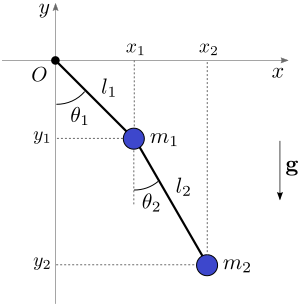
\includegraphics[scale=1]{figures/double-pendulum.png}
    \caption{A visualization of a double pendulum}
    \label{fig:1}
\end{figure}

\subsection{Results from the first set of initial conditions}\label{subsec:results-from-the-first-set-of-initial-conditions}
\begin{figure}[H]
    \centering
    \begin{subfigure}[b]{0.49\textwidth}
        \centering
        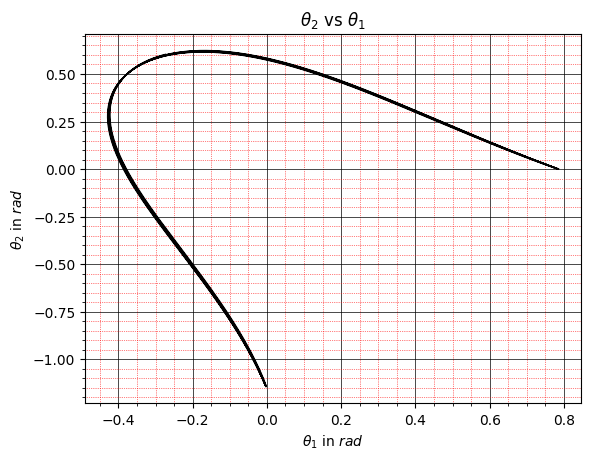
\includegraphics[width=\textwidth]{figures/initial-conditions-a/theta_2 vs theta_1.png}
        \caption{$\theta_2$ vs $\theta_1$.}
        \label{fig:2a}
    \end{subfigure}
    \hfill
    \begin{subfigure}[b]{0.49\textwidth}
        \centering
        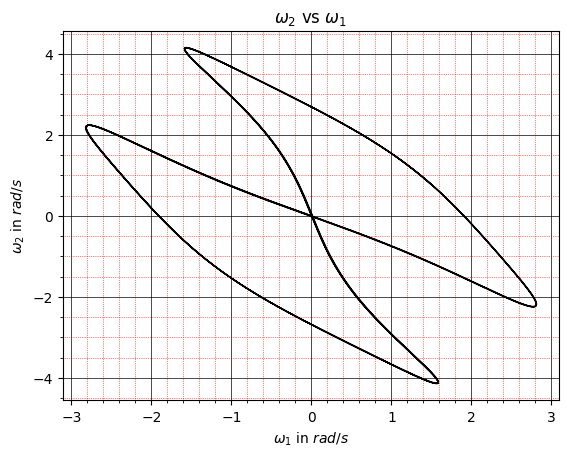
\includegraphics[width=\textwidth]{figures/initial-conditions-a/omega_2 vs omega_1.png}
        \caption{$\omega_2$ vs $\omega_1$.}
        \label{fig:2b}
    \end{subfigure}
    \hfill
    \begin{subfigure}[b]{0.49\textwidth}
        \centering
        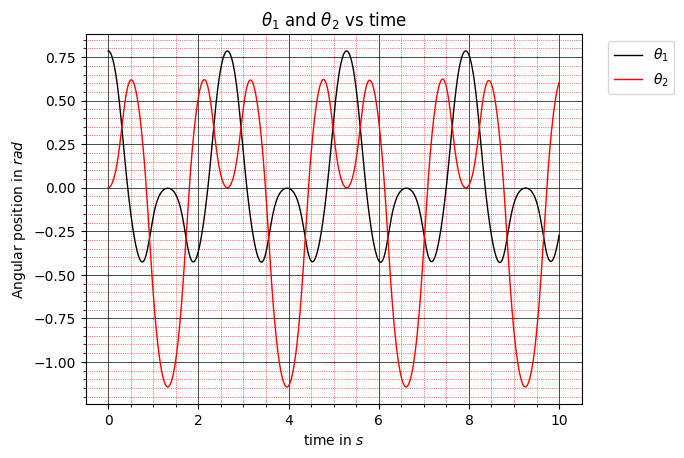
\includegraphics[width=\textwidth]{figures/initial-conditions-a/Angular Positions vs Time.png}
        \caption{$\theta_1, \theta_2$ vs time.}
        \label{fig:2c}
    \end{subfigure}
    \hfill
    \begin{subfigure}[b]{0.49\textwidth}
        \centering
        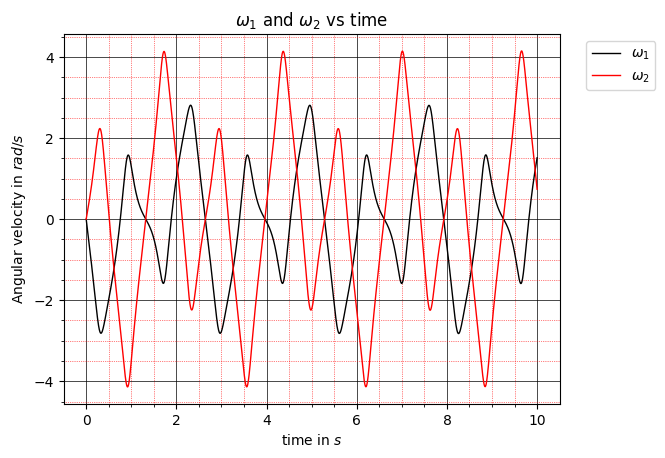
\includegraphics[width=\textwidth]{figures/initial-conditions-a/Angular Velocities vs Time.png}
        \caption{$\omega_1, \omega_2$ vs time.}
        \label{fig:2d}
    \end{subfigure}
    \hfill
    \begin{subfigure}[b]{0.49\textwidth}
        \centering
        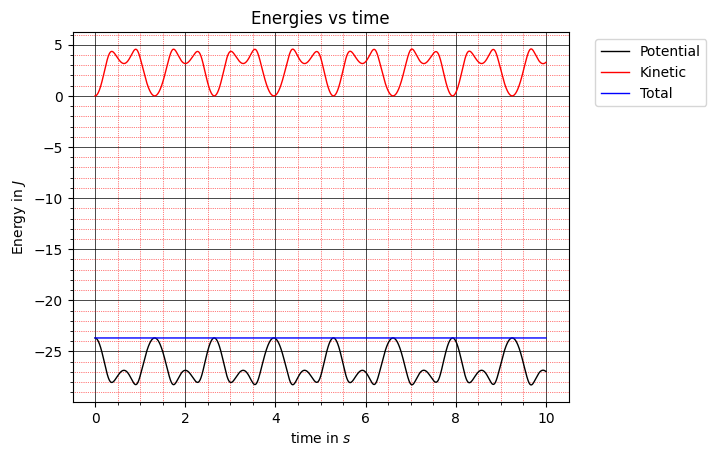
\includegraphics[width=\textwidth]{figures/initial-conditions-a/Energies vs Time.png}
        \caption{Potential, Kinetic, and Total Energies vs time.}
        \label{fig:2e}
    \end{subfigure}
    \caption{Solving the system from $t_1 = 0\text{ s}$ to $t_2 = 10\text{ s}$ where $m_1 = 1\text{ kg}$, $m_2 = 1\text{ kg}$, $l_1 = 1\text{ m}$, $l_2 = 1\text{ m}$, $\theta_{1,0} = 45^\circ$, $\theta_{2,0} = 0^\circ$, $\omega_{1,0} = 0^\circ\text{/s}$, $\omega_{2,0} = 0^\circ\text{/s}$.}
    \label{fig:2}
\end{figure}

\subsection{Results from the second set of initial conditions}\label{subsec:results-from-the-second-set-of-initial-conditions}
\begin{figure}[H]
    \centering
    \begin{subfigure}[b]{0.49\textwidth}
        \centering
        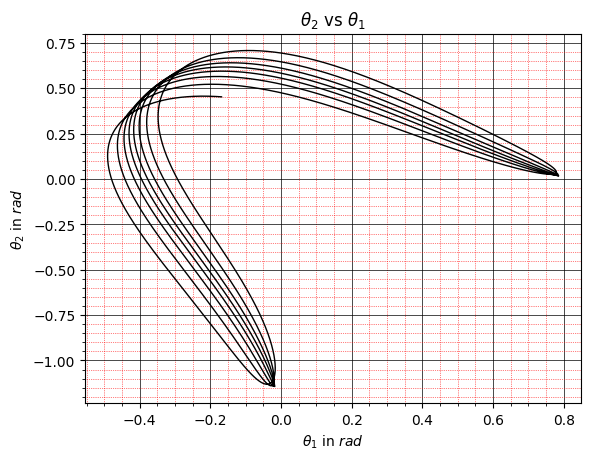
\includegraphics[width=\textwidth]{figures/initial-conditions-b/theta_2 vs theta_1.png}
        \caption{$\theta_2$ vs $\theta_1$.}
        \label{fig:3a}
    \end{subfigure}
    \hfill
    \begin{subfigure}[b]{0.49\textwidth}
        \centering
        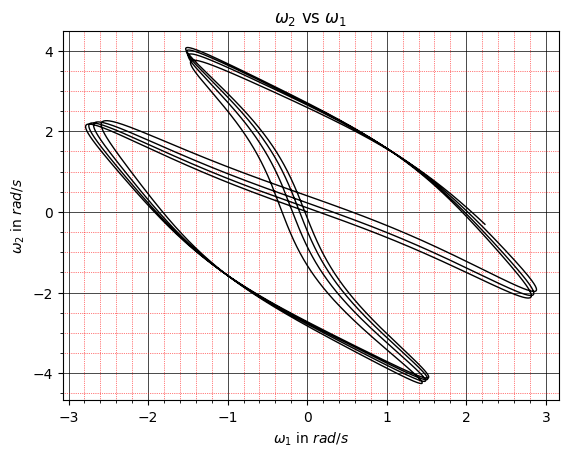
\includegraphics[width=\textwidth]{figures/initial-conditions-b/omega_2 vs omega_1.png}
        \caption{$\omega_2$ vs $\omega_1$.}
        \label{fig:3b}
    \end{subfigure}
    \hfill
    \begin{subfigure}[b]{0.49\textwidth}
        \centering
        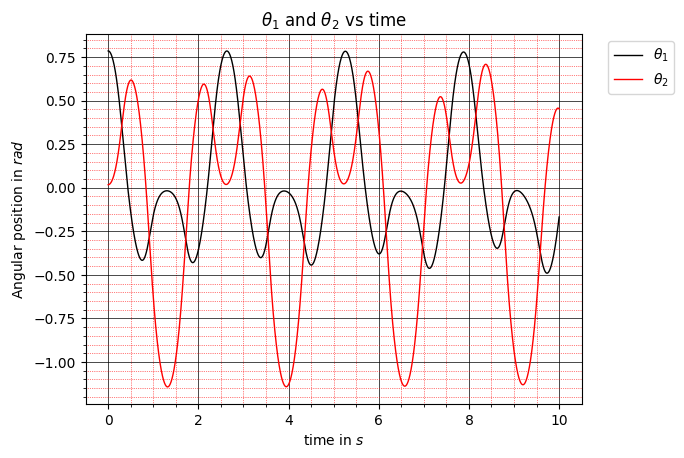
\includegraphics[width=\textwidth]{figures/initial-conditions-b/Angular Positions vs Time.png}
        \caption{$\theta_1, \theta_2$ vs time.}
        \label{fig:3c}
    \end{subfigure}
    \hfill
    \begin{subfigure}[b]{0.49\textwidth}
        \centering
        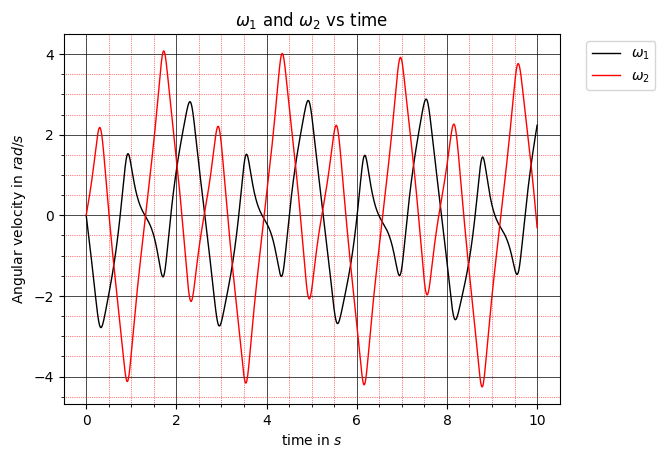
\includegraphics[width=\textwidth]{figures/initial-conditions-b/Angular Velocities vs Time.png}
        \caption{$\omega_1, \omega_2$ vs time.}
        \label{fig:3d}
    \end{subfigure}
    \hfill
    \begin{subfigure}[b]{0.49\textwidth}
        \centering
        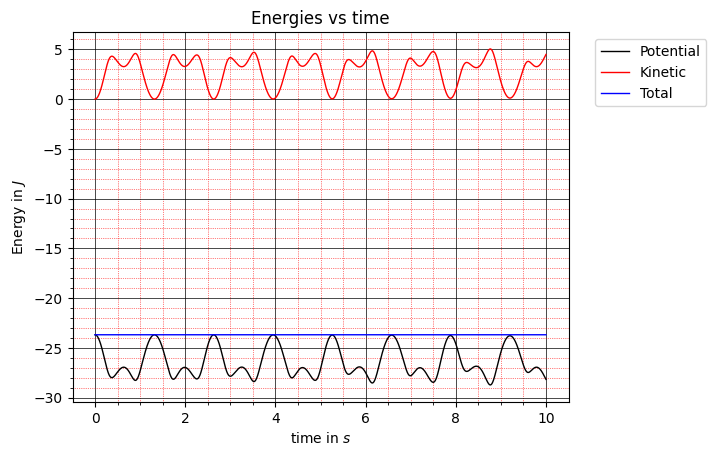
\includegraphics[width=\textwidth]{figures/initial-conditions-b/Energies vs Time.png}
        \caption{Potential, Kinetic, and Total Energies vs time.}
        \label{fig:3e}
    \end{subfigure}
    \caption{Solving the system from $t_1 = 0\text{ s}$ to $t_2 = 10\text{ s}$ with the same intial conditions from Figure~\ref{fig:2} but with $\theta_{2,0} = 0^\circ$ instead.}
    \label{fig:3}
\end{figure}

    \section{Python code}
\lstset{style=mystyle}

\subsection{System of Ordinary Differential Equations}
\label{subsec:system-of-ordinary-differential-equations}
\begin{lstlisting}[language=Python]
def df(F, t, params) -> np.array:
    # Unpack variables
    theta_1: float = F[0]
    theta_2: float = F[1]
    omega_1: float = F[2]
    omega_2: float = F[3]

    # Unpack parameters
    m_1: float = params[0]
    m_2: float = params[1]
    l_1: float = params[2]
    l_2: float = params[3]
    g: float = params[4]

    # System of differential equations
    theta_1_t: float = omega_1
    theta_2_t: float = omega_2

    # Breaking down each component since the expression is too big
    A1: float = -g * (2 * m_1 + m_2) * np.sin(theta_1)
    A2: float = - m_2 * g * np.sin(theta_1 - 2 * theta_2)
    A3: float = - 2 * m_2 * np.sin(theta_1 - theta_2)
    A4: float = (omega_2 ** 2) * l_2 + (omega_1 ** 2) * l_1 * np.cos(theta_1 - theta_2)
    B: float = l_1 * (2 * m_1 + m_2 - m_2 * np.cos(2 * (theta_1 - theta_2)))
    omega_1_t: float = (A1 + A2 + A3 * A4) / B

    # Breaking down each component since the expression is too big
    C1: float = 2 * np.sin(theta_1 - theta_2)
    C2: float = (omega_1 ** 2) * l_1 * (m_1 + m_2)
    C3: float = g * (m_1 + m_2) * np.cos(theta_1)
    C4: float = (omega_2 ** 2) * l_2 * m_2 * np.cos(theta_1 - theta_2)
    D: float = l_2 * (2 * m_1 + m_2 - m_2 * np.cos(2 * (theta_1 - theta_2)))
    omega_2_t: float = C1 * (C2 + C3 + C4) / D
    return np.array([theta_1_t, theta_2_t, omega_1_t, omega_2_t], dtype=float)
\end{lstlisting}

\subsection{My Implementation of the Runge-Kutta Order 4 Method}
\label{subsec:my-implementation-of-the-runge-kutta-order-4-method}
\begin{lstlisting}[language=Python]
def rk4(df, r, ts, h, params):
    rs = [r]
    for i in range(1, len(ts)):
        f1 = df(rs[i - 1], ts[i - 1], params)
        f2 = df(rs[i - 1] + (h / 2) * f1, ts[i - 1] + (h / 2), params)
        f3 = df(rs[i - 1] + (h / 2) * f2, ts[i - 1] + (h / 2), params)
        f4 = df(rs[i - 1] + h * f3, ts[i - 1] + h, params)
        r = rs[i - 1] + (h / 6) * (f1 + 2 * f2 + 2 * f3 + f4)
        rs.append(r)
        pass
    return get_data(rs)
\end{lstlisting}

\subsection{Helper Function}
\label{subsec:get-data-helper-function}
\begin{lstlisting}[language=python]
def get_data(data):
    rs, cs = len(data), len(data[0])
    temp = np.empty((cs, rs), dtype=float)
    for r in range(0, rs):
        for c in range(0, cs):
            temp[c][r] = data[r][c]
            pass
        pass
    if len(temp) == 1:
        return temp[0]
    return temp
\end{lstlisting}

\end{document}
